\chapter{Implementation}
\label{chap:implementation}

\section{Chosen Software Architecture}
In the given setting, the most accessible frontend is commonly a JavaScript web application.

To still make the classification run as quickly and efficiently as possible, a C++ binary runs
in the backend providing an HTTP API to the frontend application.
In order to allow for more flexibility of the HTTP server, the initial approach was to
pipe requests through a dedicated web application framework with database access
that would allow, for instance, user management next to the basic classification.
However, the resulting communication and computation overhead, even when running with very
efficient protocols such as ZeroMQ, was too high.

Extending the accessibility argument to reproducibility, Docker is a very solid choice \parencite{using-docker-in-science}.
To run the attached demo project, simply execute
\begin{minted}{bash}
  docker-compose build
  docker-compose up
\end{minted}
in the 'code' folder and point your browser to \url{https://localhost}.

\subsection{Docker Multi-Stage Build}
An enterprise-grade, scalable deployment is achieved by means of zero-dependency
Alpine Linux images which contain nothing but compiled binaries and linked libraries.

\section{The MNIST dataset}
The MNIST dataset \parencite{mnist-original} contains X train and Y test images with corresponding labels.
In order to stick to the traditional feedforward technique with data represented
in vector format, therefore it is common to reshape data from $(28, 28)$ images (represented as grayscale values in a matrix)
into a $784$ element vector.

\section{Matrix-Vector Multiplication}
The dot product that is required as part of the neural network evaluation process
needs to be implemented on SEAL ciphertexts as well.

There are multiple methods to achieve a syntactically correct dot product (matrix-vector multiplication)
as described by \textcite{2018-gazelle} for (square) matrices.

\begin{enumerate}
  \item \textbf{Naïve MatMul} - very simple to derive but impractical in practice due to the limited further
        applicability of the result consisting of multiple ciphertexts. Applicable to arbitrary matrix dimensions,
        i.e. matrices $M \in \R^{s \times t}$, of course limited by the unreasonably high memory consumption
        and computation time of this approach.
  \item \textbf{Diagonal MatMul} - a simple and practical solution applicable to square matrices $M \in \R^{t \times t}$
        that has a major advantage compared to the previous method as the computation yields a
        single ciphertext object instead of many which can be directly passed on to a following evaluation operation.
  \item \textbf{Hybrid MatMul} - essentially extending the diagonal method by generalising the definition of the
        diagonal extraction mechanism to 'wrap around' in order to match the dimensionality of the input vector.
        Applicable to arbitrary matrix dimensions, i.e. matrices $M \in \R^{s \times t}$ and favourable compared
        to the Naïve Method.
  \item \textbf{Babystep-Giantstep MatMul} - a more sophisticated technique aiming to significantly reduce the number of
        Galois rotations as they are rather expensive to carry out,
        with a performance boost especially noticeable for higher matrix dimensions.
        Without further modification, applicable to square matrices.
\end{enumerate}

For the following, define
\newcommand{\rot}{\mathrm{rot}}
\newcommand{\diag}{\mathrm{diag}}
\begin{align}
  \rot_j: \R^t \mapsto \R^t,             & \; \{\rot_j(\vec{x})\}_i = x_{i + j} \label{eq:rot-definition} \\
  \diag_j: \R^{t \times t} \mapsto \R^t, & \; \{\diag_j(M)\}_i = M_{i, (i+j)} \label{eq:diag-definition}
\end{align}
with all indices $i, j \in \Z_t$ member of the cyclic quotient group $\Z_t := \Z / t \Z$ of all integers
modulo $t$, meaning that overflowing indices simply wrap around again starting at index $0$ to simplify notation.
For the sake of compactness, we stick to this notation for the rest of this section.

\begin{figure}
  \centering
  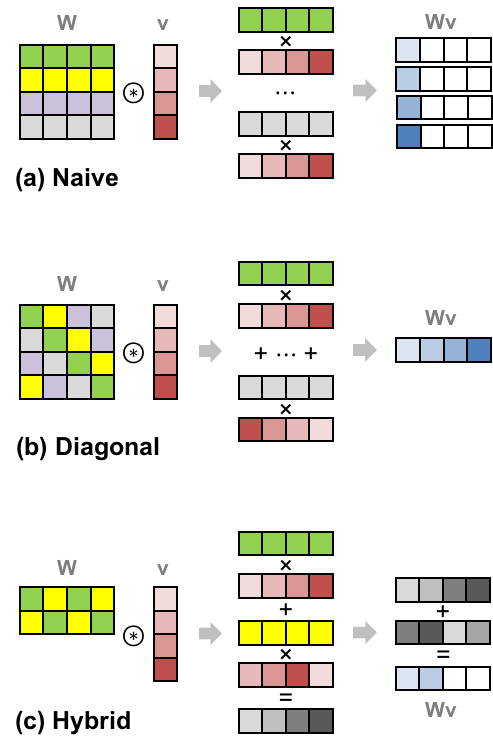
\includegraphics[width=0.4\linewidth]{figures/matrix-vector-multiplication-techniques.png}
  \caption[Image source: \cite{2018-gazelle}]{Different techniques to compute a dot product between a matrix and a vector,
    each having their up- and downsides.}
\end{figure}

\subsection{Adapting to non-square matrices}
\label{subsec:non-square-matrices}
The weight matrices in the given classification setting
are by no means square, on the contrary their output dimension tends
to be much lower than the input dimension as the goal is to reduce it from
$28^2 = 784$ to $10$ overall.

However, that also means one cannot directly apply the diagonal method
as described in the proceedings above.
This 'flaw' can be mitigated by a simple zero-padding approach
in order to make the matrix square, filling in zeroes until
the lower dimension reaches the higher one.

\subsection{The Naïve Method}
Term by term, one can express a matrix-vector product of $M \in \R^{s \times t}$ and
$\vec{x} \in \R^s$ as follows:
$$\{M \vec{x}\}_i = \sum_{j=1}^{t} M_{ij} x_j$$

Accordingly, a natural (or rather, naïve) way to model this multiplication in \textit{Microsoft SEAL}
would be to
\begin{enumerate}
  \item encode each $i$-th matrix row $(M_{i,1}, M_{i,2}, ..., M_{i,t})$ using the \cpp{Encoder}
        with matching parameters to the ciphertext of the encoded vector $\vec{x}$.
  \item multiply each encoded row with the encrypted vector using \cpp{Evaluator.multiply_plain()}
        to obtain the ciphertext vector $\vec{y_i} \in \R^s$ for row $i$.
  \item perform the 'rotate-and-sum' algorithm \parencite{2018-gazelle} on each
        resulting vector (ciphertext) $\vec{y_i}$ to obtain the actual dot product
        of the matrix row with the vector $\vec{x}$:
        \begin{enumerate}
          \item using Galois automorphisms, rotate the entries of $\vec{y_i}$ by $\frac{s}{2}$ elements
                to obtain $\rot_{\frac{s}{2}}(\vec{y_i})$.
          \item perform an element-wise sum $\vec{y_i} + \rot_{\frac{s}{2}}(\vec{y_i})$
                whose first (and also second) half now contains the sum of the two halves of $\vec{y_i}$.
          \item repeat the previous two steps $\log_2(s)$ times, halving the
                split parameter $s$ each time until one obtains $1$ element,
                which yields us the requested sum of all entries $\sum_{k=1}^s \{\vec{y_i}\}_k$
                as the dot product of $\vec{x}$ and $\vec{y_i}$.
        \end{enumerate}
  \item Given all the 'scalar' results of each row-vector dot product,
        we can construct the resulting matrix-vector product.
\end{enumerate}

\subsection{The Diagonal Method}
\begin{definition}{Diagonal Method}{diagonal-method}
  Given a matrix $M \in \R^{t \times t}$ and a vector $\vec{x} \in \R^t$,
  the dot product between the two can be expressed as
  \begin{equation}
    M \vec{x} = \sum_{i=0}^t \diag_i(M) rot_i(\vec{x})
  \end{equation}
\end{definition}

\subsection{The Hybrid Method}
To further extend the previous matrix multiplication method to solve the problem
(cf. \autoref{subsec:non-square-matrices}), it is first necessary to extend the definition of the $\diag$ operator
to non-square matrices $M \in \R^{s \times t}$.
For the following, extending the above definition:
$$\diag_j: \R^{s \times t} \mapsto \R^t, \; \{\diag_j(M)\}_i = M_{i, (i+j)}$$

To exemplarily describe an implementation of an \gls{he} algorithm, we break down the following
matrix multiplication using the method described above.
\begin{minted}{cpp}
void DenseLayer::matmulHybrid(seal::Ciphertext &in_out, const Matrix &mat, seal::GaloisKeys &galois_keys,
    seal::CKKSEncoder &encoder, seal::Evaluator &evaluator) {
  size_t in_dim = mat.shape(0);
  size_t out_dim = mat.shape(1);

  // diagonal method preparation
  std::vector<seal::Plaintext> diagonals = encodeMatrixDiagonals(mat, encoder);

  // perform the actual multiplication
  seal::Ciphertext original_input = in_out; // makes a copy
  seal::Ciphertext sum = in_out; // makes another copy
  evaluator.multiply_plain_inplace(sum, diagonals[0]);
  for (auto offset = 1ULL; offset < in_dim; offset++) {
    seal::Ciphertext tmp;
    evaluator.rotate_vector(original_input, offset, galois_keys, in_out);
    evaluator.multiply_plain(in_out, diagonals[offset], tmp);
    evaluator.add_inplace(sum, tmp);
  }
  in_out = sum;
  evaluator.rescale_to_next_inplace(in_out); // scale down once
}
\end{minted}

\subsection{The Babystep-Giantstep Optimization}
Since Galois rotations are the most computationally intensive operations in most cryptographic schemes used
today \parencite{2021-pasta}, they take a large toll on the efficiency.
In order to reduce the number of rotations required, one can make use of the \textit{Babystep-Giantstep}
optimization as described in \cite{2018-faster-helib}, which works as follows:

\begin{theorem}{Babystep-Giantstep Optimization}{bsgs}
  Given a matrix $M \in \R^{t \times t}$ and a vector $\vec{x} \in \R^t$,
  with $t = t_1 \cdot t_2$ split into two BSGS parameters $t_1, t_2 \in \N$ and
  $$\diag'_p(M) = \rot_{-\lfloor p/t_1 \rfloor \cdot t_1}(\diag_p(M))$$,
  one can express a matrix-vector multiplication as follows:
  \begin{equation}
    M \vec{x} = \sum_{k=0}^{t_2-1} \rot_{(kt_1)} \bigg(
    \sum_{j=0}^{t_1-1} \diag'_{(kt_1+j)}(M) \cdot \rot_j(\vec{x})
    \bigg)
  \end{equation}
  where $\cdot$ denotes an element-wise multiplication of two vectors.
\end{theorem}

\begin{proof}
  Starting from the adapted matrix-multiplication expression $P = (P_1, P_2, ..., P_t)^T \in \R^t$,
  we want to show that we indeed end up with an authentic matrix-vector product.
  \begin{align*}
    P = \bigg\{\sum_{k=0}^{t_2-1} \rot_{(kt_1)} \big(
    \sum_{j=0}^{t_1-1} \diag'_{(kt_1+j)}(M) \cdot \rot_j(\vec{x})
    \big)\bigg\}_i = \sum_{k=0}^{t_2-1} \sum_{j=0}^{t_1-1} m'_{kt_1+j,(i+kt_1)} x_{(i+kt_1)+j}
  \end{align*}
  with
  \begin{align*}
    m'_{p,i} = \big\{ \diag'_p(M)\big \}_i = \big\{ \rot_{-\lfloor p/t_1 \rfloor \cdot t_1}(\diag_p(M)) \big\}_i
    = M_{i-\lfloor\frac{p}{t_1}\rfloor t_1, i-\lfloor\frac{p}{t_1}\rfloor t_1 + p}
  \end{align*}
  and therefore
  \begin{align*}
    m'_{kt_1+j,i}        & = M_{i-\lfloor\frac{kt_1+j}{t_1}\rfloor t_1, i-\lfloor\frac{kt_1+j}{t_1}\rfloor t_1 + kt_1+j} \\
                         & = M_{i-kt_1-\lfloor\frac{j}{t_1}\rfloor t_1, i-kt_1-\lfloor\frac{j}{t_1}\rfloor t_1 + kt_1+j} \\
                         & = M_{i-kt_1-\lfloor\frac{j}{t_1}\rfloor t_1, i+j-\lfloor\frac{j}{t_1}\rfloor t_1}             \\
    m'_{kt_1+j,(i+kt_1)} & = M_{i+kt_1-kt_1-\lfloor\frac{j}{t_1}\rfloor t_1, i+kt_1+j-\lfloor\frac{j}{t_1}\rfloor t_1}   \\
                         & = M_{i-\lfloor\frac{j}{t_1}\rfloor t_1, i+kt_1+j-\lfloor\frac{j}{t_1}\rfloor t_1}
  \end{align*}
  leading to
  \begin{align*}
    P_i = \sum_{k=0}^{t_2-1} \sum_{j=0}^{t_1-1} m'_{kt_1+j,(i+kt_1)} x_{(i+kt_1)+j}
    = \sum_{k=0}^{t_2-1} \sum_{j=0}^{t_1-1} M_{i-\lfloor\frac{j}{t_1}\rfloor t_1, i+kt_1+j-\lfloor\frac{j}{t_1}\rfloor t_1} x_{(i+kt_1)+j}
  \end{align*}
  . Noticing that the downward rounded fraction $\lfloor\frac{j}{t_1}\rfloor$ vanishes
  in a sum with $j$ running from $0$ to $t_1-1$, we can simplify to
  \begin{align*}
    P_i = \sum_{k=0}^{t_2-1} \sum_{j=0}^{t_1-1} M_{i,i+kt_1+j} x_{i+kt_1+j}
  \end{align*}
  which contains two sums running to $t_1$ and $t_2$ respectively, containing an expression
  of the form $k \cdot t_1 + j$, which allows us to condense the nested sums into one single
  summation expression, as $$\sum_{k=0}^{t_2-1} \sum_{j=0}^{t_1-1} f(kt_1+j) = \sum_{l=0}^{t-1} f(l)$$
  indeed catches every single value $l \in \{0, 1, 2, ..., t=t_1 \cdot t_2\}$ with $l = kt_1+j$. \\
  In summary, we obtain
  \begin{align*}
    P_i & = \sum_{k=0}^{t_2-1} \sum_{j=0}^{t_1-1} M_{i,i+kt_1+j} x_{i+kt_1+j} \\
        & = \sum_{l=0}^{t-1} M_{i,i+l} x_{i+l}
    = \sum_{\nu=0}^{t-1} M_{i,\nu} x_{\nu}                                    \\
        & = \big\{M \vec{x}\big\}_i
  \end{align*}
  which indeed equals the conventional definition of a matrix-vector product.
\end{proof}

Note that the optimized matrix-vector multiplication only requires $t_1 + t_2$ as
we can store the $t_1$ inner rotations of the vector $x$ for the upcoming evaluations.
For larger matrices and vectors (larger $t$), $t_1 + t_2$ are indeed much smaller than
the conventional number of required rotations in the Diagonal or Hybrid method for instance
which was the point of this modification in the first place.

\section{Polynomial Evaluation}
From the implementation perspective, there are three properties to watch out for when
working with SEAL ciphertexts:

\begin{enumerate}
  \item Scale (retrieved using \cpp{x.scale()})
        \begin{quote}
          Scale has nothing to do with noise. "Scale out of bounds" can appear even if noise is extremely low. Although repeated multiplication of a ciphertext by a plaintext will slowly increase the noise, it is not the reason why you see "scale out of bounds".
          "Scale out of bounds" error specifically means that the scale of a ciphertext or plaintext is larger than the product of all elements in coeff\_modulus. If you perform multiplications without rescaling, you can quickly see this error. The more rescaling you perform, the less elements will be left in coeff\_modulus. Even if you managed to have the same scale in a ciphertext after every multiplication and rescale, eventually the coeff\_modulus can be too small to accommodate another multiplication.
        \end{quote}
        % https://github.com/microsoft/SEAL/issues/182#issuecomment-646234787

        Can be adjusted with: \cpp{evaluator.rescale_inplace()}
  \item Encryption Parameters (retrieved using \cpp{x.parms_id()}) \\
        Can be adjusted with: \cpp{evaluator.mod_switch_to_inplace()}
  \item Ciphertext Size (retrieved using \cpp{x.size()}) \\
        Can be adjusted with: \cpp{evaluator.relinearize_inplace()}
\end{enumerate}

\paragraph{Multiplication}
Each time one multiplies two ciphertexts, the scales multiply (logarithmically, they add up, i.e. the bits are added together).
The chain index reduces by 1. The chain index of an encoded ciphertext depends on the coeff moduli.
There must be enough bits remaining to perform the multiplication, namely log2(scale) bits.

\paragraph{Addition}
The scales must be the same, but luckily they will not change.

\section{Transparent Ciphertext}
\begin{quote}
  The problem is that you are subtracting a ciphertext from itself.
  This kind of operation results in a ciphertext that is identically zero;
  this is called a transparent ciphertext. Such a transparent ciphertext
  is not considered to be valid because the ciphertext reveals its underlying plaintext to anyone who sees it,
  even if they don't have the secret key.
  By default SEAL throws an exception when such a situation is encountered to protect you from a problem you may not have noticed.
  If you truly know what you are doing and want to enable the creation of transparent ciphertexts,
  you can configure SEAL [...].
  \parencite{kim-laine-on-transparent-ciphertexts}
\end{quote}

% https://github.com/microsoft/SEAL/issues/276#issuecomment-777073477
'transparent ciphertexts (a.k.a. ciphertexts whose second polynomial is zero) are malformed and do not need the secret key to decrypt'
